

\section{Condicions atmosfèriques a la Terra} \label{sec:cond_atmos_terra}

Primerament, és important conèixer l'atmosfera que envolta la Terra. Aquesta atmosfera es divideix en diferents capes que presenten diferents propietats \cite{nasa_atmosfera}.

\begin{figure}[h]
    \centering
    \includegraphics[width=0.75\textwidth]{imagenes/00_general/capes_atmosferiques.jpg}
    \caption{Capes atmosfèriques de la Terra. Crèdits: \cite{nasa_atmosfera}}
    \label{fig:capes_atmosferiques}
\end{figure}

\begin{itemize}
    \item \textbf{Troposfera} \\
    La troposfera s’inicia a la superfície terrestre i s’estén entre 8 i $12 \ \kilo\meter$ d’alçada. Aquesta part de l’atmosfera és la més densa. Conté el $99\%$ del vapor d'aigua del planeta. A la troposfera, les temperatures solen disminuir a mesura que s'augmenta l'alçada, ja que la major part de la calor que es troba a la troposfera es genera per la transferència d’energia a partir de la superfície de la Terra. La troposfera és la capa atmosfèrica més densa, comprimida pel pes de la resta de l’atmosfera per sobre d’aquesta. Gairebé tot els fenòmens meteorològics ocorren en aquesta regió.

    \item \textbf{Estratosfera} \\
    L’estratosfera comença just per sobre de la troposfera i s’estén fins a $50 \ \kilo\meter$ d’alçada. A l'estratosfera s'ubica la famosa capa d'ozó de la Terra, que protegeix als éssers vius de les radiacions ultraviolades del Sol. A causa de la radiació ultraviolada, la temperatura augmenta amb un augment d'alçada.

    \item \textbf{Mesosfera} \\
    La mesosfera s’inicia just per sobre de l’estratosfera i s’estén fins a 85 quilòmetres d’alçada. La temperatura a la mesosfera disminueix progressivament amb l’altitud. De fet, la part superior d’aquesta capa és la capa amb menor temperatura que es troba dins del sistema terrestre, amb una temperatura mitjana d’uns $-85^\circ C$. La majoria de meteors es cremen en aquesta capa atmosfèrica.

    \item \textbf{Termosfera} \\
    La termosfera comença just per sobre de la mesosfera i s’estén fins a 700 $\kilo\meter$ d’alçada. En aquesta capa, les temperatures augmenten amb l'altitud a causa de la baixa densitat de molècules d'aire. Aquesta capa està exempt de vapors i de núvols. En aquesta capa es produeixen els fenòmens d'aurora boreals i l'aurora austral. L’Estació Espacial Internacional orbita a la termosfera.

    \item \textbf{Exosfera} \\
    Situada entre uns 700 i 10000 $\kilo\meter$ sobre la superfície terrestre. L'exosfera és la capa més alta de l'atmosfera terrestre i, a la part superior, es fusiona amb el vent solar. La densitat de molècules en aquesta capa és extremadament baixa de manera que aquesta capa ja no es comporta com un gas sinó que les partícules s’escapen a l’espai. La majoria de satèl·lits terrestres orbiten a l’exosfera.
\end{itemize}

A continuació, s'elaboraran les diferents distribucions de pressió, temperatura i densitat a la Terra. Posteriorment, serviran de suport per explicar els comportaments les diferents gràfiques.

\subsection{Distribució de temperatura}
\begin{figure}[h]
    \centering
    \includegraphics[width=0.75\textwidth]{imagenes/03_grafiques_general/temperatura_earth.pdf}
    \caption{Representació gràfica de la distribució temperatura $T$ respecte l'altura $h$ a la Terra}
    \label{fig:temperatura_earth}
\end{figure}

La distribució de la temperatura segueix el model de capes desenvolupat en el fonament teòric \ref{tab:altituds} amb gradients lineals. La validesa del model es troba entre la superfície de la Terra i els 117776 m.

\newpage
\subsection{Distribució de pressió}
A continuació es presenta el model de pressió de l'atmosfera terrestre.\newline
Els primers 20 km són d'especial interès pel món aeronàutic i, per tant, es separarà la distribució en dos grups per a una millor visualització de l'evolució amb l'altitud.
\begin{figure}[ht]
    \centering
    \includegraphics[width=0.56\textwidth]{imagenes/03_grafiques_general/pressure_0_20_km_earth.pdf}
    \caption{Representació gràfica de la distribució pressió $p_\infty$ respecte l'altura $h$ a la Terra en un rang de $0 < h < 20 \ \kilo\meter$}
    \label{fig:pressure_0_20_km_earth}
\end{figure}

\begin{figure}[ht]
    \centering
    \includegraphics[width=0.56\textwidth]{imagenes/03_grafiques_general/pressure_20_120_km_earth.pdf}
    \caption{Representació gràfica de la distribució pressió $p_\infty$ respecte l'altura $h$ a la Terra en un rang de $20 < h < 120 \ \kilo\meter$}
    \label{fig:pressure_20_120_km_earth}
\end{figure}

\clearpage
\subsection{Distribució de densitats}
\begin{figure}[ht]
    \centering
    \includegraphics[width=0.75\textwidth]{imagenes/03_grafiques_general/density_earth.pdf}
    \caption{Representació gràfica de la distribució de densitat $T$ respecte l'altura $h$ a la Terra}
    \label{fig:density_earth}
\end{figure}

En el cas de la densitat la variació respecte el nivell del mar ja és unes 10 vegades més petita a una altura de 20 km. A més a més, a partir dels 40 km és tant baixa que, en casos on no es requereixi molta precisió, es podria aproximar a la nul·litat. 

\newpage
\section{Condicions atmosfèriques a Mart}

El procediment seguit no és només vàlid per a la Terra. Seguint un procediment similar amb l'atmosfera marciana, es poden obtenir totes les gràfiques. Com a exemple, a continuació es calculen les propietats termodinàmiques a partir de \cite{nasa_mars_sheet}.

\begin{figure}[ht]
    \centering
    \begin{minipage}{.5\textwidth}
        \centering
        \includegraphics[width=1\linewidth]{imagenes/11_mars/temperatura.pdf}
        \captionof{figure}{Distribució de temperatura}
        \label{fig:11mars}
    \end{minipage}%
        \begin{minipage}{.5\textwidth}
        \centering
        \includegraphics[width=1\linewidth]{imagenes/11_mars/densidad.pdf}
        \captionof{figure}{Distribució de densitats}
        \label{fig:12mars}
    \end{minipage}
    \begin{minipage}{.5\textwidth}
        \centering
        \includegraphics[width=1\linewidth]{imagenes/11_mars/pressio_0_20.pdf}
        \captionof{figure}{Distribució de pressió $0-20$ km}
        \label{fig:13mars}
    \end{minipage}%
        \begin{minipage}{.5\textwidth}
        \centering
        \includegraphics[width=1\linewidth]{imagenes/11_mars/pressio_20_120.pdf}
        \captionof{figure}{Distribució de pressió $20-120$ km}
        \label{fig:14mars}
    \end{minipage}
\end{figure}

Les distribucions de temperatura i pressió a Mart es recullen segons \cite{nasa_mars_info}:
\begin{itemize}
    \item Per $h > 7000 \ \meter$
    \begin{align*}
        T &= -23.4 - 0.00222 h \\
        P &= 0.699 * \exp{\left( -0.00009 h \right)}
    \end{align*}
    \item Per $h \leq 7000 \ \meter$
    \begin{align*}
        T &= -31 - 0.000998 h \\
        P &= 0.699 * \exp{\left( -0.00009 h \right)}
    \end{align*}
\end{itemize}

\newpage
\section{Entrada balística a la Terra}
\subsection{Gràfica: Velocitat respecte Altitud}

La gràfica \ref{fig:velocitat} representa la velocitat del vehicle en front a la l'alçada. Si s'analitza amb detall aquesta gràfica, per una $\beta=500$ per una alçada de prop dels $80 \cdot 10^3 \ \meter$ a mesura que disminueix s'alçada la velocitat es manté gairebé constant a un valor d'aproximadament $7000 \ \meter\second$. A mesura que es disminueix l'alçada, la velocitat del vehicle segueix disminuint de forma bruscament en quan s'assoleix una alçada de $50 \cdot 10^3 \ \meter$ on seguidament comença un tram en què aquesta relació pren una forma lineal. No és estrany aquest canvi de comportament ja que com s'ha vist en l'apartat \ref{sec:cond_atmos_terra}, l'estratosfera se situa per sobre de la troposfera i s'estén fins a prop dels $50 \ \kilo\meter$ d'alçada. 

\begin{figure}[ht]
    \centering
    \includegraphics[width=0.75\textwidth]{imagenes/01_ballistic_graficas/velocitat.pdf}
    \caption{Representació gràfica de la velocitat $v$ respecte l'alçada $h$ per diferents coeficients balístics $\beta$}
    \label{fig:velocitat}
\end{figure}

A partir de la troposfera ($\sim 12 \ \kilo\meter$) els valors de la velocitat per $\beta=500$ i $\beta=1000$ canvien de pendent i la velocitat sembla estabilitzar-se al voltant de $300 \meter/\second$. En canvi, si el vehicle tingués un alt coeficient balístic, aquesta estabilitat no es presenta en cap moment i la velocitat a $0 \meter$ és superior a $2800 \meter/\second$, el qual suposa que no ha estat capaç e vehicle de frenar-se suficient i la inviabilitat d'aquesta $\beta$.

A mesura que disminueix el coeficient balístic, per una mateixa alçada la velocitat del vehicle amb major coeficient balístic és més gran que el del vehicle amb menor coeficient balístic tal i com s'ha comentat anteriorment. De fet, menor coeficient balístic es tradueix com un augment de l'àrea de la secció transversal o un augment de la resistència aerodinàmica $C_D$, llavors $BC$ disminueix. De tal manera que la desacceleració és major.

\newpage
\subsection{Gràfica: Desacceleració respecte Altitud}
La desacceleració és un cas especial d’acceleració pel qual només s’aplica a objectes que perden velocitat amb el temps. Per tant, és la velocitat amb què s’alenteix un objecte.

L'acceleració és un vector que indica la com varia la velocitat en magnitud amb un direcció concreta. En un cas de moviment unidimensional, s'utilitzen signes negatius i positius per indicar la direcció. Així, si els signes són negatius, l'objecte es va desaccelerant. La desacceleració és, per tant, l'acceleració amb un signe negatiu. 

\begin{figure}[ht]
    \centering
    \includegraphics[width=0.75\textwidth]{imagenes/01_ballistic_graficas/desacceleracio.pdf}
    \caption{Representació gràfica de la desacceleració $a$ respecte l'alçada $h$ per diferents coeficients balístics $\beta$}
    \label{fig:desacceleracio}
\end{figure}

En la reentrada balística, noteu com a mida que minva l'alçada, el vehicle va adquirint desacceleració paulativament fins arribar a un pic en què la desacceleració és màxima. Aquest pic es troba a una alçada de $\sim 30 \kilo\meter$ (pel cas de $\beta = 100$ coincideix just amb el punt d'inflexió de la gràfica anterior [Figura \ref{fig:velocitat}]. Si es continua disminuint l'alçada, s'observa com la desacceleració continua decaient tendint cada cop cap a un valor de desacceleració nul·la.

Tanmateix, és interessant destacar que, si s'augmenta el coeficient balístic, el màxim de desacceleració es trasllada cada cop a una alçada menor. Aquest fenomen coincideix amb el resultat de la gràfica \ref{fig:velocitat} i el seu significat físic s'explica perquè en augmentar el coeficient balístic, és a dir, una disminució del $C_D$ i/o de l'àrea $S$ significa que el coeficient balístic $\beta$ augmenta i per conseqüent, la desacceleració del vehicle disminueix. Cal destacar també com per una $\beta=5000$, la desacceleració màxima és més petita que els els casos de menor $\beta$, la qual cosa és coherent perquè ndica que li costa més frenar-se al vehicle.

\newpage
\subsection{Gràfica: Pressió dinàmica respecte altitud}
La pressió es defineix com una força per àrea d’unitat. Quan s'exerceix una força sobre un objecte, aquesta força s'aplica sobre una superfície en concret. La pressió relaciona aquestes due variables. En el cas de fluids, són les molècules d'aire que exerceixen una pressió sobre la superfície considerada. Cal distingir entre dos tipus de pressió:
\begin{itemize}
    \item Pressió estàtica: És la pressió aplicada per l’aire i actua de forma normal a la superfície del cos.
    \item Pressió dinàmica: És la pressió associada a l’energia cinètica de l’aire que impacta sobre la superfície considerat. Aquesta es pot expressar com:
    \begin{equation}
        q = \frac{1}{2} \rho v^2
    \end{equation}
\end{itemize}
Quan un fluid es troba en moviment, la inèrcia del moviment provoca un increment addicional de la pressió estàtica al xocar sobre la secció perpendicular al moviment. La pressió dinàmica depèn de la velocitat i la densitat del fluid.

A continuació es mostra la gràfica \ref{fig:pressio_dinamica} associat a la pressió dinàmica del vehicle respecte l'alçada. En primer lloc, cal destacar l'odre de magnitud de la pressió dinàmica, la qual es troba al voltant de $\sim 10^6$. 

\begin{figure}[ht]
    \centering
    \includegraphics[width=0.75\textwidth]{imagenes/01_ballistic_graficas/pressio_dinamica.pdf}
    \caption{Representació gràfica de la pressió dinàmica $q$ respecte l'alçada $h$ per diferents coeficients balístics $\beta$}
    \label{fig:pressio_dinamica}
\end{figure}

Pel que fa referència a la pressió dinàmica, en enginyeria aeroespacial existeix un punt on es maximitza l'estrès aerodinàmic en una nau espacial en el vol atmosfèric. En altres paraules, sota el punt de màxima Q, l'efecte de l'acceleració de la nau espacial per crear més pressió dinàmica s'imposa a l'efecte de la reducció de densitat de l'aire. Per tant, ariba un punt en què la relació és màxima. Passant el punt màxim, aquesta es redueix en la mesura que es redueix la velocitat.

\newpage
\subsection{Gràfica: Mach respecte Altitud}

Respecte a la gràfica del Mach, el comportament d'aquest coeficient adimensional ve descrit per la següent relació:
\begin{equation} \label{eq:mach_definition}
    M = \frac{v}{a}
\end{equation}
on $M$ és el número de Mach, $v$ és la velocitat del vehicle i $a$ és la velocitat del so.
La velocitat del so $a$ és un paràmetre que depèn de diversos variables com el tipus de medi en què es propaga el so i la temperatura del medi de tal forma que, partint de l'equació de la conservació de la quantitat de moviment s'arriba a:
\begin{equation*}
    a = \sqrt{\left( \frac{\partial p}{\partial \rho}\right)_s}
\end{equation*}
Assumint que el gas és caloríficament perfecte. Per tal cas, la relació isentròpica és:
\begin{equation*}
    \frac{p_1}{p_2} = \left(\frac{\partial p}{\partial \rho}\right)^\gamma
\end{equation*}
Es pot obtenir que, la velocitat del so:
\begin{equation*}
    a = \sqrt{\frac{\gamma p}{\rho}}
\end{equation*}
A primera vista l'equació superior sembla indicar que la velocitat del so depèn de la pressió i densitat, tanmateix, introduint l'equació d'estat pels gasos ideals $P=\rho R_g T$:
\begin{equation}
    a = \sqrt{\gamma R T}
\end{equation}
L'expressió resultant es tracta de la relació de la velocitat del so per un gas caloríficament perfecte i és funció només de la temperatura $T$ i del tipus de medi en què viatja.
\cite{anderson}.

\begin{figure}[ht]
    \centering
    \includegraphics[width=0.75\textwidth]{imagenes/01_ballistic_graficas/mach.pdf}
    \caption{Representació gràfica del número de Mach $M$ respecte l'alçada $h$ per diferents coeficients balístics $\beta$}
    \label{fig:mach}
\end{figure}

De tal forma que, per una alçada del voltant dels $80 \ \kilo\meter$,
ens situem sobre la capa de la mesosfera on la temperatura i amb l'alçada. Segons la gràfica \ref{fig:temperatura_earth}, aquesta és la capa amb menys temperatura amb un $190 \ \kelvin$. Relacionant aquest número adimensional amb la velocitat, és fàcil deduir que s'arribin a números de Mach elevats de magnituds superiors a $M=20$. Vegeu que en aquesta alçada, la velocitat de reentrada del vehicle és molt elevat i la temperatura del medi molt baix, amb la qual cosa, la relació $\frac{v}{a}$ es dispara.
Al voltant de l'alça de $30 \ \kilo\meter$ es produeix un canvi i l número de Mach disminueix intensament en qüestió de $20 \ \kilo\meter$ i passa a prendre un valor d'entre $M=5$ i $M=10$. En aquest tram la caiguda del número de Mach pren la mateixa forma que la caiguda de la velocitat doncs, la influència del canvi de temperatures és menyspreable en front al canvi de velocitats.


\subsection{Gràfica: Reynolds respecte Altitud}
Si un objecte es desplaça a través de l'atmosfera, les molècules de gas de l'atmosfera properes a l'objecte es veuen pertorbades per aquest. En aquesta interacció es generen forces aerodinàmiques entre el gas i l’objecte.
El nombre de Reynolds expressa la relació de forces inercials (forces associades a la resistència al moviment) amb les forces viscoses (forces adherents) \cite{kundu}:
\begin{equation}
    Re = \frac{\text{Forces inercials}}{\text{Forces viscoses}}
\end{equation}

La magnitud d’aquestes forces depenen de la forma de l’objecte $d$, la velocitat de l’objecte $v$, la densitat del fluid que interacciona amb l’objecte i d’altres dues propietats com són la viscositat cinemàtica $\mu$. 

Anàlogament, partint d'un anàlisi detallat de l'equació de la conservació de la quantitat de moviment. Les forces inercials es caracteritzen pel producte de la densitat $\rho$ per la velocitat $u$ i pel gradient de la velocitat $\frac{\partial V}{\partial x}$
Les forces viscoses es caracteritzen pel coeficient de viscositat dinàmica $\mu$ pel segon gradient de la velocitat $\mu \dfrac{ \partial^2 u}{\partial x^2}$. 
El número Reynolds Re es converteix llavors en:
\begin{equation*}
    Re = \frac{\rho u \dfrac{\partial u}{\partial x}}{\mu \dfrac{ \partial^2 u}{\partial x^2}}
\end{equation*}
Desenvolupant, el gradient de la velocitat és proporcional a la velocitat dividida per una longitud característica $L$. Paral·lelament, la segona derivada de la velocitat és proporcional a la velocitat dividida pel quadrat la longitud característica, donant:
\begin{equation}
    Re = \frac{\rho u L}{\mu}
\end{equation}

\begin{figure}[ht]
    \centering
    \includegraphics[width=0.75\textwidth]{imagenes/01_ballistic_graficas/reynolds.pdf}
    \caption{Representació gràfica del número de Reynolds $Re$ respecte l'alçada $h$ per diferents coeficients balístics $\beta$}
    \label{fig:reynolds}
\end{figure}

En quant al comportament del número de Reynolds, a la mesosfera ($\sim 50 - 85\ \kilo \meter$) la densitat de d'aire és molt reduïda. L’aire de la mesosfera té una densitat extremadament baixa: el $99.9\%$ de la massa de l’atmosfera es troba per sota de la mesosfera. Com a resultat, el número de Reynolds és relativament baix en comparació amb les altres corbes. Nogensmenys, en un anàlisis detallat el valor del Reynolds més reduït de tots els coeficients balístics, això és, $\beta=100$ es troba a l'ordre de $4\cdot10^5$ . Aquest valor és similar per la resta de corbes a una alçada elevada. Tot seguit, aquesta tendència es veu afectat per l'imminent augment de la densitat que passa de de ser d'aproximadament $\sim 0.0020 \ \kilo\gram / \meter^3$ a augmentar en aproximadament un $200 \%$ fins a un valor de $\sim 0.3639 \ \kilo\gram / \meter^3$ a la troposfera ($\sim 11 \ \kilo\meter$).

A mesura que augmenta el coeficient balístic, com s'ha vist amb les gràfiques del Mach i velocitat respecte l'altura. La velocitat també augmenta. Com s'ha explicat anteriorment, en augmentar el coeficient balístic, es redueix el $C_D$. Aleshores, degut la pèrdua de la força de resistència aerodinàmica els efectes de fregament entre el vehicle i els gasos també disminueixen. En conseqüència, aquest fenomen afecta negativament a la velocitat doncs perilla la frenada. Anàlogament a \ref{fig:pressio_dinamica}, el número de Reynolds també depèn de la densitat i el quadrat de la velocitat, tot introduint la viscositat dinàmica.


\newpage
\subsection{Gràfica: Pressió d'estancament respecte Altitud}
Es defineix la temperatura d'estancament com la temperatura que tindria un fluid si es portés al repòs ($v=0 \ \meter/\second$) adiabàticament. La pressió d'estancament és la pressió que obtindria el fluid si es portés aquest isentròpicament ($\dd S = 0$) fins al repòs (adiabàtic i reversible).

L'ús de propietats d'estancament com la temperatura o la pressió d'estancament proporcionen una mesura de la quantitat d’energia total o capacitat d'accelerar el flux disponible. Les propietats d’estancament no són les ``reals'' (exceptuant els llocs en què la velocitat sí són nules). Les propietats estàtiques són les reals. 
La densitat de l’aire, la velocitat del so depenen de les propietats estàtiques locals.

El tub de pitot és instrument usat en aviació per mesurar les pressions estàtiques i dinàmiques. Coneixent aquestes dues pressions és fàcil trobar la pressió d'estancament. Aplicant l'equació de Bernouilli \cite{anderson_2},
\begin{equation*}
    P_1 + \frac{1}{2} \rho v^2_1 = p_2 + \frac{1}{2} \rho v^2_2
\end{equation*}
Aplicant en una línia de corrent en els punts $A$ i $B$ s'obté:
\begin{equation}
    \underbrace{P_1}_{\substack{\text{Pressió} \\ \text{estàtica}}} + \underbrace{\frac{1}{2} \rho v^2_1}_{\substack{\text{Pressió} \\ \text{dinàmica}}} = \underbrace{p_0}_{\substack{\text{Pressió} \\ \text{d'estancament}}}
\end{equation}

\begin{figure}[ht]
    \centering
    \includegraphics[width=0.75\textwidth]{imagenes/01_ballistic_graficas/pressio_estancament.pdf}
    \caption{Representació gràfica de la pressió d'estancament $P_t$ respecte l'alçada $h$ per diferents coeficients balístics $\beta$}
    \label{fig:pressio_estancament}
\end{figure}

Particularment, la pressió estàtica en el nostre problema es tracta de la pressió atmosfèrica a cada alçada la qual segueix les Figures \ref{fig:pressure_0_20_km_earth} i \ref{fig:pressure_20_120_km_earth}. La pressió dinàmica, en canvi, és la associada al moviment de les partícules de 'aire al xocar amb el vehicle. Aleshores, la pressió total d'estancament és la suma de les dues anteriors. Tanmateix, aquest és només és vàlid per règim incompressible. En canvi, per un règim de flux compressible, això és, per un $M>0.3$ cal reformular les expressions. 

Finalment, la pressió d'estancament es tracta d'una propietat intensiva del fluid i dóna a conèixer del nivell d'energia d'aquest. A més a més, alhora és un indicador del nivell de compressió del fluid.

A l'hora d'aplicar aquesta definició, cal diferenciar quin règim de treball s'està considerant \cite{cumpsty}.
\begin{itemize}
    \item Règim Subsònic [$M<1$] \\
    En aquest règim es fa servir l'expressió del flux per un flux isentròpic
    Partint de l'equació de conservació de l'energia:
    \begin{equation}
        \frac{T}{T_0} = 1 + \frac{\gamma - 1}{2} M^2
    \end{equation}
    Aplicant les relacions isentròpiques,
    \begin{equation*}
        \frac{p}{\rho^\gamma} = \mathrm{const} 
        \hspace{7mm} \text{i} \hspace{7mm} 
        T p^{\frac{1 - \gamma}{\gamma}} = \mathrm{const}
    \end{equation*}
    S'obté que la pressió d'estancament s'expressa de la següent forma:
    \begin{equation}
        \frac{p_0}{p_\infty} = \left( 1 + \frac{\gamma - 1}{2} M_\infty^2\right)^\frac{\gamma}{\gamma - 1}
    \end{equation}
    
    \item Règim supersònic i hipersònic [$M\geq 1$] \\
    En règim supersònic o sònic, cal considerar la possibilitat de la generació d'una ona de xoc normal. Aquest valors són obtinguts a partir de les equacions \textit{Rankine-Hugoniot} i les relacions isentròpiques:
    \begin{equation} \label{eq:rankine_hugoniot_p_shock}  
        p_{shock} = p_\infty \left[ 1 + \frac{2 \gamma}{\gamma  + 1} (M_\infty^2 - 1) \right]
    \end{equation}
    Introduint l'expressió anterior en les equacions de \textit{Rankine-Hugoniot} per règim sònic i supersònic la pressió d'estancament $p_0$ \cite{gallais}:
    \begin{equation} \label{eq:rankine_hugoniot_p_0}
        p_0 = p_{shock} \left[ 1 + \frac{\gamma - 1}{2} \cdot \frac{1 + \dfrac{\gamma-1}{2} M_\infty^2}{\gamma M_\infty^2 - \dfrac{\gamma-1}{2}} \right]^\frac{\gamma}{\gamma-1}
    \end{equation}
\end{itemize}

Com es pot observar en les gràfiques, el comportament global de les corbes s'assimila molt a la corba de pressions dinàmiques. No obstant, fixant-nos amb l'escala horitzontal en comparació, existeix un \textit{offset}. Com es pot observar en la gràfica, la dependència obtinguda no només depèn de la del Mach de vol, i en conseqüència de la temperatura sinó que també cal distingir entre un règim subsònic o supersònic, doncs a partir de règim supersònic pot existir ones de xoc. A mesura que s'augmenta el com
eficient balístic, el número de Mach és creixent, de forma que que els valors de pressió d'estancament són també més elevats, fins i tot arribar a l'ordre de $\sim 10^7$ en el cas de $\beta=5000$, el qual clarament indica la forta contribució d'ones de xoc.


\newpage
\subsection{Gràfica: Entalpia d'estancament respecte Altitud}
La entalpia és una propietat d'un sistema termodinàmic que es igual a l'energia interna més el producte de la pressió pel volum.
\begin{equation}
    H(S,p) = U + p V
\end{equation}
Aquesta propietat representa una mesura de la quantitat d'energia del sistema. A més a més, es tracta d'una funció d'estat amb propietats extensives, és a dir, es poden sumar diversos subsistemes modificant el valor final en funció de la grandària.
\begin{equation}
    H = \sum_k H_k
\end{equation}
on $H$ es l'entalpia total dels subsistemes, $k$ es refereix al nombre de subsistemes i $H_k$ representa cada subsistema.

La unitat de mesura de l'entalpia en el sistema internacional és el Joule $[J]$. Cal també recalcar que en sistema imperial s'utilitzen també les Unitats Tèrmiques Britàniques $BTU$ i les calories. 
En \cite{adams} s'utilitzen les BTU, que es defineixen com la quantitat de calor necessari per augmentar una lliura d'aigua un gran Fahrenheit.
Encara que l'entalpia com a valor únic ja és de força utilitat, a vegades es prefereix comptabilitzar el canvi en l'entalpia a pressió o volum constant per a simplificar l'expressió. L'entalpia total, no es pot mesurar directament i sempre s'utilitza un punt de referència ja que només el canvi té un significat físic.

L'equació de l'energia per un flux estacionari en règim permanent sense calors externs i energies internes es pot escriure com:
\begin{equation}
    h_1 + \frac{v^2_1}{2} = h_2 + \frac{v^2_2}{2}
\end{equation}
on la $h$ és l'entalpia que es pot reescriure com la capacitat calorífica a pressió constant $C_p$ per la temperatura i on $T_0$ representa la temperatura d'estancament:
\begin{equation}
    C_p T + \frac{v^2}{2} = \underbrace{C_p T_0}_{\text{$v_2 =0$}}
\end{equation}
Una altra forma d'expressar la relació anterior a partir de diferencials on cap valor es constant, ja que les propietats termofísiques dependran de l'altitud de vol.
\begin{equation}
    dH = C_p\cdot dT + V\cdot dp
\end{equation}
Els valors del coeficient $C_p$ es poden aproximar utilitzant únicament la temperatura a partir dels coeficients NASA. A continuació s'utilitzaran les taules extretes de \cite{heat_mass_transfer} per a aire sec comprès entre 100 K i 2500 K:
\begin{equation}
    C_p = 1034.09 -2.849 \cdot 10^{-1}T + 7.817 \cdot 10^{-4}T^2 - 4.971 \cdot 10^{-7}T^3 + 1.077 \cdot 10^{-10}T^4 \quad (\frac{J}{kgK})
\end{equation}
Finalment, s'obté l'equació a partir de les variables termofísiques de l'atmosfera amb les aproximacions corresponents:
\begin{equation}
    h_0 = C_p \cdot T + \frac{v^2}{2}
\end{equation}
On $h_0$ es l'entalpia d'estancament, una forma de generalitzar el concepte d'entalpia quan es treballa amb fluids amb alta energia cinètica, és a dir, amb velocitats no despreciables, com per exemple en el flux a través de turbines de gas o motors d'aviació. El balanç d'energia del fluid és considera de forma adiabàtica i reversible (isentròpicament), fins a velocitat nul·la. 

\begin{figure}[ht]
    \centering
    \includegraphics[width=0.75\textwidth]{imagenes/01_ballistic_graficas/entalpia_estancament.pdf}
    \caption{Representació gràfica de l'entalpia d'estancament $h_0$ respecte l'alçada $h$ per diferents coeficients balístics $\beta$}
    \label{fig:entalpia_estancament}
\end{figure}

La variació de l'entalpia d'estancament amb els coeficients balístics és molt notable. Per a coeficients baixos l'entalpia d'estancament es redueix més lentament que per a coeficients elevats, principalment a causa de l'altitud a partir de la qual es comença a variar el valor entalpic. Les pendents de decreixement per a qualsevol coeficient balístics són constants entre els $0.5 \frac{J}{kg}$ i els $2 \frac{J}{kg}$. Si es referencia a l'altitud a nivell del mar, les $\beta$ entre 100 i 1000 finalitzen en la mateixa posició mentre que per a $\beta = 5000 \frac{lbf}{ft^2}$, com que l'entalpia d'estancament comença a decréixer a una altura més baixa, llavors arriba al terra amb un valor aproximat de $h_o = 0.4 \quad \frac{J}{kg}$.

\newpage
\subsection{Gràfica: Transferència de calor d'estancament respecte Altitud}
L'energia cinètica d'un vehicle en reentrada es dissipa transformant l'energia tèrmica (calor) a la vegada que el sistema desaccelera.

La transferència de calor en el punt d'estancament normalment s'aproxima a partir de mètodes numèrics. Un mètode molt utilitzat és el de Fay $\&$ Ridell (1958), que es pot veure en \cite{adams}.
\begin{equation}
    \dot{q}_w=\frac{0.763}{Pr_w^{0.6}} \cdot (\rho_e\mu_e)^{0.4} \cdot (\rho_w\mu_w)^{0.1} \cdot [(h_0)_e-h_w] \cdot \left[1+(Le^{0.52}-1)\frac{h_d}{(h_0)_e}\right] \cdot \left[\left(\frac{du_e}{dx}\right)_t\right]^{0.5}
\end{equation}
Amb gairebé la mateixa precisió existeix el mètode simplificat de Sutton Graves, només valid per a la Terra i Mart, que s'utilitzarà per al càlcul del flux calorífic en \cite{aerothermodynamics}. És important recalcar que la validesa només s'aplica per a superfícies catalítiques. Existeixen altres expressions per a parets no catalítiques però no es tractaran.
\begin{equation}
    q_s = k_{world}\left(\frac{\rho}{R_n}\right)^{\frac{1}{2}} \cdot V^3
\end{equation}
on $\rho$ és la densitat, $R_n$ és l'aspror, que es considera el d'una esfera de $radi = 0.03048 m$, $V$ és la velocitat, $k_{Earth} = 1.7415 \cdot 10^{-4}$ és la constant per a la Terra i $k_{Mars} = 1.9027 \cdot 10^{-4}$ és la constant per a Mart, ambdues en unitats del SI segons la NASA \cite{aerothermodynamics}. Tot i això, es important destacar que \cite{adams} utilitza unes constants similars que són $k_{Earth} = 1.83 \cdot 10^{-4}$  i $k_{Mars} = 1.89 \cdot 10^{-4}$ per a realitzar els càlculs.

\begin{figure}[ht]
    \centering
    \includegraphics[width=0.75\textwidth]{imagenes/01_ballistic_graficas/transferencia_calor_estancament.pdf}
    \caption{Representació gràfica de la transferència de calor d'estancament $\dot{Q}$ respecte l'alçada $h$ per diferents coeficients balístics $\beta$}
    \label{fig:transferencia_calor_estancament}
\end{figure}

La transferència de calor d'estancament varia considerablement segons el coeficient balístic analitzat. Per a un $\beta = 100 \ (\frac{lbf}{ft^2})$, la $\dot{Q}$ s'incrementa entre els $76 \ \kilo\meter$ i els $35 \ \kilo\meter$ i decreix fins a una transferència nul·la entre els $35 \ \kilo\meter$ i els $20 \ \kilo\meter$. Per a la $ \beta = 500 \ (\frac{lbf}{ft^2})$ es duplica la magnitud de la transferència de calor amb un màxim de $-1.2 \enskip \frac{W}{m^2}$ a una altitud de 26 km. De manera similar, per a la $ \beta = 1000 \ (\frac{lbf}{ft^2})$ la posició de la màxima transferència es dóna a terme a una altitud més baixa amb un valor més alt de calor d'estancament. Finalment, pel coeficient balístic màxim els valors es disparen a més del doble del cas anterior en la posició de 12 km amb una transferència de calor de $-3.6 \enskip \frac{W}{m^2}$.


\subsection{Gràfica: Temps de reentrada respecte Altitud}

El temps de reentrada respecte a l'altitud es gràfica en la Figura \ref{fig:temps}.
\begin{figure}[ht]
    \centering
    \includegraphics[width=0.75\textwidth]{imagenes/01_ballistic_graficas/temps.pdf}
    \caption{Representació gràfica del temps de reentrada $t$ respecte l'alçada $h$ per diferents coeficients balístics $\beta$}
    \label{fig:temps}
\end{figure}
En aquest cas, no és d'estranyar que en augmentar el paràmetre del coeficient balístic $\beta$, la massa del vehicle s'imposa al terme del drag i l'àrea. Tot plegat, en un augment de $\beta$, disminueix el temps de reentrada arribant a valors de fins $\sim 50 \ \second$ per la $\beta = 5000$ i de fins $180 \ \second$ per una $\beta = 100$. No obstant, també cal remarcar que aquesta dependència presenta un caràcter lineal de de l'inici de $h = 76.2 \ \kilo\meter$ fins una alçada d'uns $25 - 15 \ \kilo\meter$ on es produeix un canvi en la pendent a una pendent més suau tot i conservant la linealitat.
La velocitat mitja en la primera regió és entorn a:
\begin{equation*}
    v_{\text{mitjà}} = \frac{80\cdot10^3 - 15\cdot10^3}{35} = 1857.1439 \ \meter\second = 6685.7149 \ \kilo\meter/\second
\end{equation*}
Tanmateix, avaluant la velocitat instantània, el valor mitjà s'allunya del valor de velocitat instantània real que es mostra en la gràfica \ref{fig:velocitat}. Doncs la velocitat associat a les alçades de $20 \ \kilo\meter$ fins als $76.2 \ \kilo\meter$ superen els $4000 \ \meter/\second$ (exceptuant $\beta=100$). La conclusió que s'extreu d'aquest resultat és coherent amb la definició de coeficient balístic.

\newpage
\subsection{Gràfica: Abast respecte Altitud}
L'abast és la distància màxima horitzontal que pot assolir un objecte que es llença a partir d'una determinada altitud inicial. En aquest cas tenim una reentrada d'un objecte balístic com el que utilitzaven els primers ICBM (Inter-Continental Ballistic Missiles).
\begin{figure}[ht]
    \centering
    \includegraphics[width=0.75\textwidth]{imagenes/01_ballistic_graficas/abast.pdf}
    \caption{Representació gràfica del abast $\Delta x$ respecte l'alçada $h$ per diferents coeficients balístics $\beta$}
    \label{fig:abast}
\end{figure}

Fins a una altura de 25 km, l'abast és indiferent al coeficient balístic. A partir d'aquest punt, una reentrada amb $\beta = 100 \enskip (\frac{lbf}{ft^2}$) descendeix de manera gairebé vertical fins els 260 km de distància respecte la poisició inicial. Per a valors entre $\beta = 500 \enskip (\frac{lbf}{ft^2}$) i $\beta = 5000 \enskip (\frac{lbf}{ft^2}$), aquesta separació es duu a terme a una altura 10 km inferior. Així, per a $\beta = 500 \enskip (\frac{lbf}{ft^2}$), $\beta = 1000 \enskip (\frac{lbf}{ft^2}$) i $\beta = 5000 \enskip (\frac{lbf}{ft^2}$), els valors d'abast són, respectivament, 305 0km, 320 km i 340 km.

\newpage
\subsection{Gràfica: Energia dinàmica respecte Altitud}
La energia dinàmica és una relació entre la pressió dinàmica i la velocitat d'un cos tal que:
\begin{equation}
    \text{Energia Dinàmica} = \frac{\rho \cdot V^3}{2}
\end{equation}
En una reentrada, la velocitat és el terme més important de l'energia dinàmica a causa del seu exponencial cúbic.

\begin{figure}[ht]
    \centering
    \includegraphics[width=0.75\textwidth]{imagenes/01_ballistic_graficas/energia_dinamica.pdf}
    \caption{Representació gràfica de l'energia dinàmica $E$ respecte l'alçada $h$ per diferents coeficients balístics $\beta$}
    \label{fig:energia_dinamca}
\end{figure}

Per a $\beta$ entre 100 i 500 $\frac{\mathrm{lbf}}{\mathrm{ft}^2}$ l'energia dinàmica es troba entre l'interval de 0 i $0.35 \cdot 10^{10} \enskip \frac{Pa \cdot m}{s}$. Per a $\beta = 1000$ hi ha un màxim de $0.7\cdot 10^{10} \enskip \frac{Pa \cdot m}{s}$ a una altura de 18 km. Seguint la tendència, per a $\beta = 5000$ els valors gairebé es multipliquen per 5 respecte a la $\beta$ anterior arribant a $3.3 \cdot 10^{10} \enskip \frac{Pa \cdot m}{s}$. \\
A partir dels coeficients balístics analitzats, es veu una tendència a decréixer de la posició de màxima energia dinàmica quant més gran és el coeficient balístic, amb una pèrdua d'energia considerable un cop es passa aquest valor.


\newpage
\clearpage
\section{Cas d'entrada balística a la Terra: Càpsula Mercury}

El projecte Mercury va ser el primer programa de vol espacial humà dels Estats Units. Va funcionar des del 1959 fins al 1963 amb dos objectius: posar un humà en òrbita al voltant de la Terra i realitzar-ho abans que ho aconseguís la Unió Soviètica, com a part de la carrera espacial. Aquesta càpsula va ser un èxit en la primera missió el 5 de maig de 1961 on Alan Shepard es va convertir en el primer nord-americà a l'espai en vol suborbital. No obstant això, la Unió Soviètica prèviament havia guanyat la carrera enviant a Yuri Gagarin a l'espai un mes abans.
El \textit{Friendship 7} va ser una càpsula d'un sol home amb forma de con amb un cilindre muntat a la part superior. De dos metres de llarg, $1.9$ metres de diàmetre fixada a una torre d'escapament de $5.8$ metres al cilindre de la càpsula. Per tal de d'evitar els efctes abrasius de la calor, es va cobrir amb un protector de calor ablatiu per protegir-lo contra la calor de $3000\degrees C$ en la reentrada a l’atmosfera.

\begin{figure}[ht]
    \centering
    \begin{subfigure}{.5\textwidth}
        \centering
        \includegraphics[width=0.75\linewidth]{imagenes/09_mercury_graficas/mercury_capsule.jpg}
        \caption{{Esquema de la càpsula Mercury. Crèdits: \cite{mercury_capsule}}}
    \end{subfigure}%
    \begin{subfigure}{.5\textwidth}
        \centering
        \includegraphics[width=0.75\linewidth]{imagenes/09_mercury_graficas/mercury_capsule_space.jpg}
        \caption{{Càpsula Mercury a l'espai. Crèdits: \cite{mercury_capsule_space}}}
    \end{subfigure}
\end{figure}

Per tal de fer un estudi detallat del comportament d'aquesta càpsula, calen conèixer les seves propietats:
\begin{itemize}
    \item Pes $W = 11844.720 \ \newton$
    \item Àrea de referència $A = 2.812 \ \meter^2$
    \item Longitud de referència $L = 1.890 \ \meter$
    \item Radi de punta (esfera) $R_N = 0.3048 \ \meter$
    \item Coef. Sustentació $C_L = 0 $
    \item Coef. Drag $C_D = 1.60 $
\end{itemize}
Amb aquestes dades s'obté un coeficient balístic de $\beta=54.98 \mathrm{lb_f}/{ft}^2$ o en $\mathrm{SI}$ $\beta \approx 2632$.
\begin{itemize}
    \item Alçada inicial $h_0 \approx 85344 \ \meter$
    \item Velocitat inicial $v_0 = 7010.4 \ \meter/\second$
    \item Angle d'entrada $\gamma = 1.5 \degrees$
\end{itemize}

Els resultats obtinguts es mostren a la Figura \ref{fig:mercury_capsule}. Començant per la gràfica de la velocitat respecte l'altitud, el comportament segueix essent similar a l'anàlisi de la secció anterior. A mesura que disminueix en alçada, es va reduint la velocitat. A més, torna a evidenciar-se una zona lineal.

Pel que fa al temps de reentrada, la tendència de la corba es pot aproximar lineal i en qüestió de $\approx 6$ minuts arriba a la Terra. Aquest comportament es respalda degut que té un coeficient balístic de només $\beta=54.98$, quasi la meitat de la menor $\beta$ de les gràfica \ref{fig:temps}. Estant aquest temps en caiguda lliure no és estranyar que l'abast sigui de $1000 \ \kilo\meter$.

El pic de desacceleració, en canvi, no arriba a als valors de $>20 g$ sinó que el seu màxim es troba a quasi $10 g$. Que en comparació amb les dades oficials no s'allunyen massa dels $8 \ g$ que va patir John Gleen. Tot i això, posteriorment s'observarà que la reentrada sustentadora ofereix valors molt inferiors, la qual cosa per és un gran avantatge si la missió és tripulada.

Finalment, en relació al número de Mach, cal insistir en què la major part del trajecte és vol supersònic, i aquest disminueix progressivament amb l'alçada, de tal manera que és a patir de l'altura mitja de l'estratosfera quan la disminució creix de forma més agressiva, tal i com s'ha comentat anteriorment \ref{fig:mach}.

\clearpage
\subsection{Entrada balística de la càpsula Mercury ``Friendship 7'' a la Terra}

\begin{figure}[ht]
    \centering
    \begin{subfigure}{.37\textwidth}
        \centering
        \includegraphics[width=\linewidth]{imagenes/09_mercury_graficas/velocitat_no_title.pdf}
        \caption{Velocitat $V$ ($\meter/\second$)}
    \end{subfigure}%
    \begin{subfigure}{.37\textwidth}
        \centering
        \includegraphics[width=\linewidth]{imagenes/09_mercury_graficas/temps_no_title.pdf}
        \caption{Temps de reentrada $t$ ($\second$)}
    \end{subfigure}
    % Siguiente línea
        \begin{subfigure}{.37\textwidth}
        \centering
        \includegraphics[width=\linewidth]{imagenes/09_mercury_graficas/abast_no_title.pdf}
        \caption{Abast $\Delta x$ ($\meter$)}
    \end{subfigure}%
    \begin{subfigure}{.37\textwidth}
        \centering
        \includegraphics[width=\linewidth]{imagenes/09_mercury_graficas/desacceleracio_no_title.pdf}
        \caption{Desacceleració $a$ ($g$)}
    \end{subfigure}
    % Siguiente línea
        \begin{subfigure}{.37\textwidth}
        \centering
        \includegraphics[width=\linewidth]{imagenes/09_mercury_graficas/mach_no_title.pdf}
        \caption{Número de Mach $M$ ($adim$)}
    \end{subfigure}%
    \caption{Trajectòria de reentrada balística a la Terra de la càpsula Mercury}
    \label{fig:mercury_capsule}
\end{figure}

Aquestes gràfiques s'obtenen particularitzant les entrades balístiques per les propietats especifiques de la càpsula Mercury "Friendship" a partir de l'atmosfera USA 1976. Un important factor que es pot observar que el Coronel Glenn va estar subjecte a una càrrega de desacceleració per sobre de 8g durant un període de temps aproximat de 30 segons. \newline
Aquesta va ser la raó principal que va promoure el desenvolupament de les reentrades sustentadores per a viatges espacials tripulats de manera que la càrrega de g durant períodes llargs de temps.

\newpage
\section{Entrada sustentadora a la Terra}

Com s'ha explicat anteriorment, el cas de l'Space Shuttle, és un exemple de vehicle en què usa una reentrada sustentadora.

Així doncs, a continuació s'estudiaran trajectòries d'entrada representatives a la Terra per tres valors inicials de l'angle d'entrada $\gamma_0$ ($0.1$ , $1.0$ i $2.5$ $^\circ$). Les condicions inicials de la reentrada són:
\begin{itemize}
    \item Alçada inicial $h_0 = 76200 \ \meter$
    \item Velocitat inicial $v_0 = 7010.4 \ \meter/\second$
\end{itemize}
Els paràmetres disseny de l'Space Shuttle són els següents:
\begin{itemize}
    \item Pes $W = 889644 \ \newton$
    \item Àrea de referència $A = 819.912 \ \meter^2$
    \item Longitud de referència $L = 32.766 \ \meter$
    \item Radi de punta (esfera) $R_N = 0.3048 \ \meter$
    \item Coef. Sustentació $C_L = 0.84 $
    \item Coef. Drag $C_D = 0.84 $
\end{itemize}

Amb aquestes dades, el coeficient balístic resultant és de $\beta = 4237.401 \newton/\meter^2$ ($\beta=88.5 \mathrm{lb_f}/\mathrm{ft^2}$ en Sistema Imperial). Els càlculs s'han realitzat amb el coeficient de reentrada de $\beta=88.5$ per obtenir els càlculs amb més precisió. 
La transferència de calor per una esfera amb nas radial de $R_N = 0.3048$ usant la correlació de Sutton-Graves. El número de Reynolds es calcula amb la longitud de referència superior, aquesta longitud és bàsicament la longitud de l'Space Shuttle. Tal i com es mostra en les Figures \ref{fig:angle_lift}, per una eficiència aerodinàmica de l'ordre de la unitat és molt sensible a l'angle d'entrada. 

\begin{figure}[ht]
    \centering
    \begin{subfigure}{.5\textwidth}
        \centering
        \includegraphics[width=\linewidth]{imagenes/02_lifting_graficas/angle_descens_vs_temps.pdf}
        \caption{Angle de descens ($\degrees$) vs. temps ($s$)}
        \label{fig:angle_descens_vs_temps_aaaaaaaaaaaa}
    \end{subfigure}%
    \begin{subfigure}{.5\textwidth}
        \centering
        \includegraphics[width=\linewidth]{imagenes/02_lifting_graficas/angle_descens_vs_altitud.pdf}
        \caption{Angle de descens ($\degrees$) vs. altitud ($m$)}
        \label{fig:angle_descens_vs_altitud_aaaaaaaaaaa}
    \end{subfigure}
    \caption{Variació dels angles de descens amb el temps i l'altitud}
    \label{fig:angle_lift}
\end{figure}

\noindent
La entrada amb un angle de reentrada massa elevat resulta en una trajectòria oscil·latòria a elevades altituds, fins i tot incloent la possibilitat de retornar a l'espai exterior. En el cas de la entrada balística, en canvi, un increment en l'angle de reentrada resultava en un decreixement en el temps de reentrada i del rang.

La variació de l'angle influeix principalment a la desacceleració, la pressió dinàmica, la transferència de calor d'estancament i l'energia dinàmica.

\newpage
\subsection{Gràfica: Velocitat respecte Altitud}

\begin{figure}[ht]
    \centering
    \includegraphics[width=0.75\textwidth]{imagenes/02_lifting_graficas/velocitat.pdf}
    \caption{Representació gràfica de la velocitat $V$ respecte l'alçada $h$ per diferents coeficients balístics $\beta$}
    \label{fig:velocitat_lift}
\end{figure}

La velocitat per a un angle $\gamma_o = 0.1 \degrees $ té un pendent aproximadament constant des de l'altitud inicial fins els 45 km. En canvi, per l'angle $\gamma_o = 1.0 \degrees $, la velocitat es veu alterada amb una sinusoïdal amb un coeficient d'esmorteïment. De forma similar, per l'angle $\gamma_o = 2.5 \degrees $, la velocitat varia considerablement fins els 45 km amb un interval de valors de dimensions considerables.\newline
A partir dels 45 km, l'angle no interfereix en la variació de la velocitat fins que l'objecte arriba a la superfície terrestre.
\newpage
\subsection{Gràfica: Desacceleració respecte Altitud}

\begin{figure}[ht]
    \centering
    \includegraphics[width=0.75\textwidth]{imagenes/02_lifting_graficas/desacceleracio.pdf}
    \caption{Representació gràfica de la desacceleració $a$ respecte l'alçada $h$ per diferents coeficients balístics $\beta$}
    \label{fig:desacceleracio_lift}
\end{figure}

La desacceleració presenta un esquema complex per a altituds superiors als 34 km. Entre el valor inicial i els 34 km, la desacceleració s'incrementa fins a quadruplicar el valor inicial. Per a $\gamma_o = 0.1 \degrees $ existeixen petites variacions però es podria aproximar a una equació de segon grau tal que la $\text{desacceleració} = h^2+h_i$. Per a $\gamma_o = 1.0 \degrees $, com s'ha vist a les gràfiques \ref{fig:angle_lift}, el valor de $\gamma$ influeix fortament sobre la desacceleració provocant un moviment oscil·latori característic fins a l'altitud prèviament esmentada. \newline
Per evitar aquest fenomen, es recomana utilitzar angles petits, concretament inferiors a $1 \degrees$, que minimitzen l'oscil·lació del conjunt.

Un factor important per una vol tripulat és la reducció significativa de les càrregues $g$ en la reentrada sustentadora versus la entrada balística. Per exemple, per la reentrada sustentadora del Space Shuttle, els astronautes experimenten una desacceleració del voltant de $0.5 - 1 g$ comparats amb els $8 g$ de la càpsula Mercury.

\newpage
\subsection{Gràfica: Pressió dinàmica respecte Altitud}

\begin{figure}[ht]
    \centering
    \includegraphics[width=0.75\textwidth]{imagenes/02_lifting_graficas/pressio_Dinamica.pdf}
    \caption{Representació gràfica de la pressió dinàmica $q$ respecte l'alçada $h$ per diferents coeficients balístics $\beta$}
    \label{fig:pressio_dinamica_lift}
\end{figure}

La pressió dinàmica segueix la mateixa tendència que la desacceleració a causa de la influencia de $\gamma$ en els resultats. Es segueix veient un oscil·lador esmorteït en sentit vertical que disminueix entre el punt inicial i els 32 km, a partir dels quals existeix una independència de l'angle en la pressió dinàmica. També es compleix que per a angles majors la inestabilitat és més gran. \newline
Fins a un angle $\gamma = 1.0 \degrees$ les variacions es podrien considerar controlables però per a angles $\gamma = 2.5 \degrees$ o superiors les variacions poden arribar als $4000$ Pa.
\newline Es recomanaria un estudi acurat per a mantenir un angle on les variacions de pressions al llarg del temps fossin mínimes de manera que la integritat de l'aeronau no es pogués veure afectada.

\newpage
\subsection{Gràfica: Número de Mach respecte Altitud}

\begin{figure}[ht]
    \centering
    \includegraphics[width=0.75\textwidth]{imagenes/02_lifting_graficas/mach.pdf}
    \caption{Representació gràfica del número de Mach $M$ respecte l'alçada $h$ per diferents coeficients balístics $\beta$}
    \label{fig:mach_lift}
\end{figure}

El número de Mach inicial $ M = 25$ denota una velocitat de reentrada atmosfèrica gairebé lineal per $\gamma_o = 0.1 \degrees $ fins a una altitud de 48 km. Pels altres dos angles, el número de Mach té el mateix comportament que la velocitat en aquest interval com es d'esperar. La zona altament hipersònica, entre $M = 10$ i $M = 25$ és on es produeixen variacions considerables mentre que per la zona hipersònica, entre $M =5$ i $M= 10$, el comportament és linealitzable pels angles d'estudi.\newline
La part supersònica, que considerarem entre $M=1.2$ i $M = 5$, es troba entre les altituds de 25 km i 42 km, la part transsònica, entre $M=0.8$ i $M=1.2$, es troba entre les altituds de 18 km i 25 km i, finalment, l'estat subsònic des de 18km fins a la superfície terrestre. És important recalcar que la velocitat en la superfície no es nul·la.

\newpage
\subsection{Gràfica: Número de Reynolds respecte Altitud}

\begin{figure}[ht]
    \centering
    \includegraphics[width=0.75\textwidth]{imagenes/02_lifting_graficas/reynolds.pdf}
    \caption{Representació gràfica del número de Reynolds $Re$ respecte l'alçada $h$ per diferents coeficients balístics $\beta$}
    \label{fig:reynolds_lift}
\end{figure}

El número de Reynolds és invariant amb els angles $\gamma$ d'estudi. Això es fàcilment visible si estudiem les variables de les quals depèn:
\begin{equation}
    Re = \frac{\rho \cdot v_s \cdot L_{car}}{\mu}
\end{equation}
La densitat i la viscositat dinàmica només depenen de les propietats termofísiques de l'atmosfera, que són constants diferents conegudes per a cada altitud. Per una altra banda, la longitud característica només depèn del objecte i es manté constant en aquest cas. \newline
Per tant, la única variable que podria modificar el resultat seria la velocitat però com els números de Reynolds de la reentrada son de l'ordre de $10^7$, l'efecte de petites variacions en la velocitat no és apreciable. \newline
El rang entre $Re = 0$ i $Re = 11$ es podria aproximar a una exponencial negativa a partir de la qual el rang fins a $Re = 16$ és una recta de pendent constant.

\newpage
\subsection{Gràfica: Pressió d'estancament respecte Altitud}

\begin{figure}[ht]
    \centering
    \includegraphics[width=0.75\textwidth]{imagenes/02_lifting_graficas/pressio_estancament_no_title.pdf}
    \caption{Representació gràfica de la pressió d'estancament $p_0$ respecte l'alçada $h$ per diferents coeficients balístics $\beta$}
    \label{fig:pressio_estancament_lift}
\end{figure}

Excepte en la regió entre $80$ km i $50$ km, la pressió d'estancament es manté constant per a qualsevol angle de descens. En aquesta primera zona, els angles $\gamma = 0.1 \degrees$ i $\gamma = 1.0 \degrees$ proporcionen resultats aproximats mentre que $\gamma = 2.5 \degrees$ visualitza el comportament oscil·lant característic dels vehicles sustentadors. 

El valor inicial és gairebé nul a causa de que la pressió i la densitat ho són també. A mesura que disminueix augmenta la pressió i la densitat mentre que disminueix la velocitat, tot i això, la pressió es va incrementant de forma gairebé exponencial negativa fins arribar a la superfície.


\newpage
\subsection{Gràfica: Transferència de calor respecte Altitud}

\begin{figure}[ht]
    \centering
    \includegraphics[width=0.75\textwidth]{imagenes/02_lifting_graficas/transferencia_calor.pdf}
    \caption{Representació gràfica de la pressió d'estancament $q$ respecte l'alçada $h$ per diferents coeficients balístics $\beta$}
    \label{fig:transf_calor_lift}
\end{figure}

Un factor molt important en l'entrada sustentadora té a veure amb el pic de la màxima transferència de calor. Contràriament al cas balístic en què el màxim es situa per baixes altituds, normalment per sota dels $30 - 45 \ \kilo\meter$ d'alçada, per l'entrada sustentadora, en canvi, el màxim es troba per damunt dels $60 \ \kilo\meter$ d'alçada.

Això comporta unes conseqüències importants en el sistema de protecció tèrmica ja que una prioritat és que la nau mantingui la integritat de la calor durant la reentrada i sigui capaç d'absorbir tot el flux de calor de calor durant la reentrada.

També és important recalcar el model d'oscil·lador harmònic que segueixen els angles $\gamma = 1.0 \degrees$ i $\gamma = 2.5 \degrees$ entre les posicions inicials i els 46 km a causa de la dependència amplificada de $\gamma$ a mesura que va augmentant l'angle.

\newpage
\subsection{Gràfica: Temps de reentrada respecte Altitud}

\begin{figure}[ht]
    \centering
    \includegraphics[width=0.75\textwidth]{imagenes/02_lifting_graficas/temps.pdf}
    \caption{Representació gràfica del temps de reentrada $t$ respecte l'alçada $h$ per diferents coeficients balístics $\beta$}
    \label{fig:temps_lift}
\end{figure}

El temps de reentrada total varia entre $t=1350$ i $t=1500$ segons l'angle inicial. Evidentment, per angles més petits trigarà més temps ja que l'abast és superior. La zona que comprèn els valors des de l'inici fins els 50 km actuen com a ones sinusoïdals amb esmorteïment que depèn de l'angle inicial. A partir d'aquest punt les línies son paral·leles localment independentment de l'angle d'estudi. En aquest cas, les variacions de les magnituds generals no es desplacen entre grans intervals com en casos anteriors on la dependència de $\gamma$ és major.

\newpage
\subsection{Gràfica: Abast respecte Altitud}

\begin{figure}[ht]
    \centering
    \includegraphics[width=0.75\textwidth]{imagenes/02_lifting_graficas/abast.pdf}
    \caption{Representació gràfica de l'abast $\Delta x$ respecte l'alçada $h$ per diferents coeficients balístics $\beta$}
    \label{fig:abast_lift}
\end{figure}

L'abast es veu clarament minvat per a angles majors. Tal i com s'esperaria en un planejador a la l'atmosfera baixa terrestre, per a angles petits com ,per exemple, l'angle $\gamma = 0.1 \degrees$, l'abast es veu incrementat uns 800 km respecte de l'angle $\gamma = 2.5 \degrees$. En un punt mig, més aprop, de l'angle mínim es troba $\gamma = 1.0 \degrees$ amb uns 1900 km d'abast.

A partir dels 40 km cap a la superfície terrestre, l'abast es comporta de forma independent a l'angle $\gamma$ però si ens fixem en la part superior torna a haver l'oscil·lador harmònic característic de les gràfiques amb sustentació.

\newpage
\subsection{Gràfica: Energia dinàmica respecte Altitud}

\begin{figure}[ht]
    \centering
    \includegraphics[width=0.75\textwidth]{imagenes/02_lifting_graficas/energia_dinamica.pdf}
    \caption{Representació gràfica de l'energia dinàmica $E$ respecte l'alçada $h$ per diferents coeficients balístics $\beta$}
    \label{fig:energia_dinamica_lift}
\end{figure}

En aquest cas analitzarem cada angle per separat ja que les diferencies són notables.
L'energia dinàmica inicial a $\gamma = 0.1 \degrees$ es va incrementant fins els 59 km d'altitud i després comença a decréixer fins que arriba a la superfície terrestre. Les oscil·lacions són relativament petites i es podrien menysprear.

Per a $\gamma = 1.0 \degrees$ les oscil·lacions són molt visibles i l'energia dinàmica del sistema varia gairebé un màxim d'$1 \enskip \pascal \cdot \meter / \second$. De la mateixa manera, en el cas de $\gamma = 2.5 \degrees$, el sistema varia gairebé un màxim de $3 \enskip \pascal \cdot \meter / \second$ i oscil·la descontroladament.








